\documentclass[tikz,border=4pt]{standalone}
\begin{document}
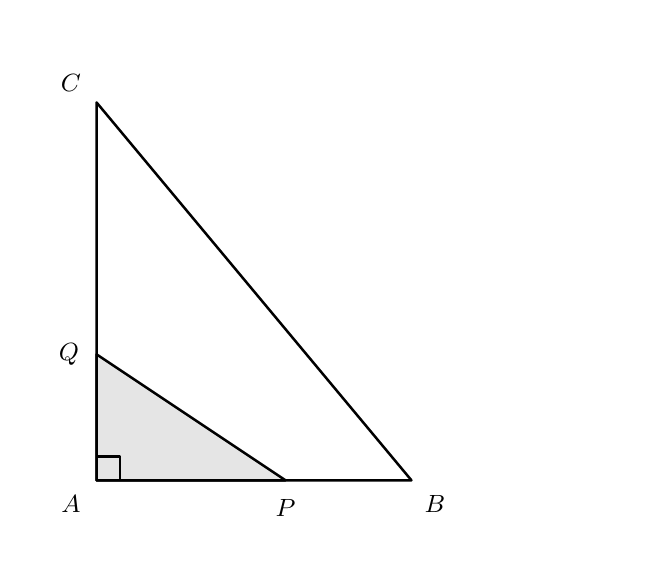
\begin{tikzpicture}[x=0.025cm,y=-0.025cm]
\path[use as bounding box] (0,0) rectangle (300,265);
\path[draw=black,fill=none,line width=0.8999999999999999pt,line join=round] (35,230) -- (195,230) -- (35,38) -- cycle;
\path[draw=black,fill=gray!20,line width=0.8999999999999999pt,line join=round] (35,230) -- (131,230) -- (35,166) -- cycle;
\path[draw=black,fill=none,line width=0.8999999999999999pt,line join=round] (35,218) -- (47,218) -- (47,230);
\node[font=\small,inner sep=0pt] at (22,242) {$A$};
\node[font=\small,inner sep=0pt] at (207,242) {$B$};
\node[font=\small,inner sep=0pt] at (22,28) {$C$};
\node[font=\small,inner sep=0pt] at (131,244) {$P$};
\node[font=\small,inner sep=0pt] at (21,166) {$Q$};
\end{tikzpicture}
\end{document}
